 \documentclass[a4paper, 12pt]{article}
\usepackage[left=2.5cm, right=2.5cm,top=2.5cm,text ={18cm,25cm}]{geometry}
\usepackage[utf8]{inputenc}
\usepackage{times}
\usepackage{enumitem}
\usepackage{graphicx}
\usepackage{hhline}
\usepackage{pdflscape}
\usepackage{afterpage}
\usepackage{svg}
\usepackage{changepage}
\usepackage{amsmath}
\usepackage{adjustbox}
\newcommand\blankpage{%
    \null
    \thispagestyle{empty}%
    \addtocounter{page}{-1}%
    \newpage}

\renewcommand{\contentsname}{Obsah}

\begin{document}
\begin{center} 
\thispagestyle{empty}
\Huge
\textsc{Fakulta informačních technologií\\Vysoké učení
technické v Brně}\\
\vspace{\stretch{0.167}}


\includegraphics[scale = 0.5]{fit-logo.eps}

\vspace{\stretch{0.215}}

\LARGE Dokumentace k prvnímu projektu předmětu IPK\\
\Huge Varianta 2: Klient-server pro jednoduchý přenos souborů \\
\vspace{\stretch{0.218}}
\Huge
Petr Knetl  \\
\LARGE
(xknetl00)
\vspace{\stretch{0.400}}
\end{center}
{\LARGE \hfill
7. března 2018}

\newpage

\tableofcontents
\pagenumbering{arabic}
\thispagestyle{empty}
\setcounter{page}{1}
\newpage

\section{Zadání}
Zadáním bylo navrhnout a implementovat jednoduchý aplikační protokol architektury klient-server pro přenos souboru. Soubor je možné přenášet jak z klienta na server, tak i ze serveru ke klientovi.

\section{Implementace}
Implementace je rozdělena do dvou aplikací, jedna pro klienta a druhá pro server. Soubory jsou v obouch směrech přesouvány po packetech o velikosti \emph{256 bajtů}. K přenosu souboru je využit \emph{TCP protokol} s \emph{blokujícími sockety}.

\subsection{aplikace serveru}
Server je spuštěn s jedním povinným parametrem, s číslem portu. Při spuštění inicializuje zdroje a vytváří socket pro navazování komunikace se serverem. Poté v nekonečné smyčce čeká dokud se klient nepokusí navázat komunikaci. K ukončení serveru dochází pouze zasláním SIGINT signálu.

Při úspěšném navázání komunikace s klientem je vytvořeno nový proces pro jeho obsluhu. Pokud již dochází ke komunikace mezi serverem a jiným klientem, nově vzniklý proces čeká na konec jejich komunikace.

Jakmile je proces na řadě, vytváří druhý socket pro přenos dat. Poté čte ze strany klienta textovou zprávu, která  blíže specifikuje navázané spojení. Ze zprávy získává  název přenášeného souboru a informaci o tom zda se bude ze serveru číst, nebo na něj ukládat.  Dále v případě  zápisu na server je vytvořenen nový soubor. Pokud soubor s tímto názvem již existuje, je přepsán. Pokud se klient pokouší ze severu kopírovat neexistující soubor, tak proces odesílá klientovi informaci o neexistujícím souboru a končí chybovou hláškou. Soubor se vždy ukládá do pracovního adresáře serveru.

\subsubsection{Konečný automat serveru}
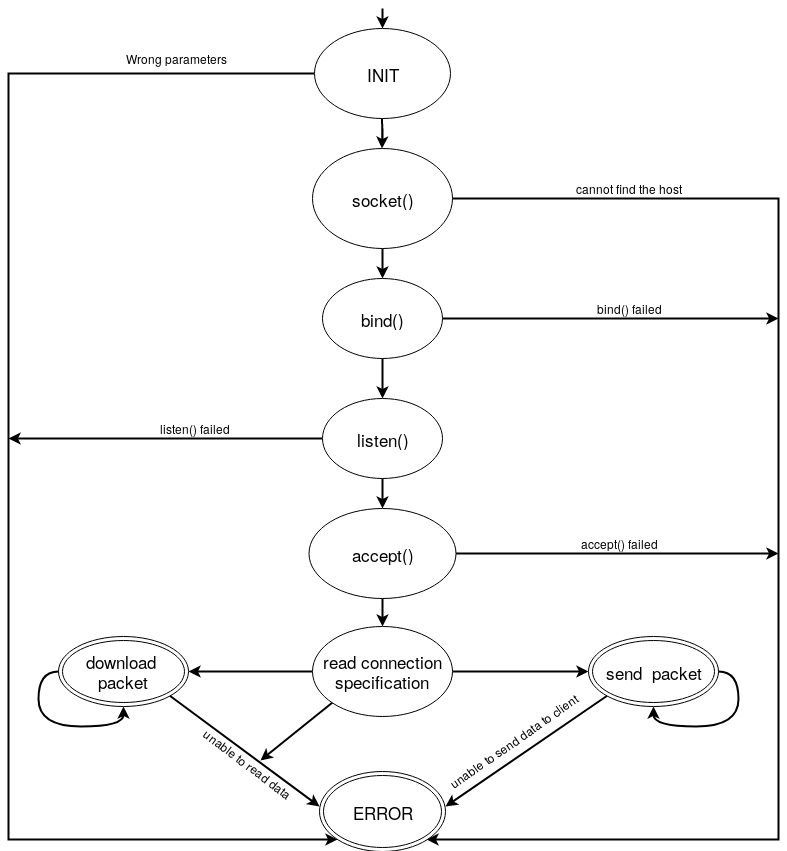
\includegraphics[scale = 0.5]{IPK_FSMSERVER.png}
\subsection{aplikace klienta}
Klient je spuštěn s třemi povinnými parametry (název hosta serveru, číslo portu a názvem souboru ke čtení/odeslání). Klient inicializuje spojení se serverem skrze uvedený port. 

Pokud klient čte soubor ze serveru, tak vytváří nový soubor v cestě zadané parametrem do kterého data ukládá. Pokud soubor již existuje, je přepsán.  Pokud soubor na straně serveru neexistuje, klient přijímá tuto informaci a končí s chybovou hláškou. V případě zápisu na server klient ověří zda soubor existuje. Pokud ano, posílá data serveru. Po dokončení posílání/příjmu dat klient končí.

\subsubsection{Konečný automat klienta}
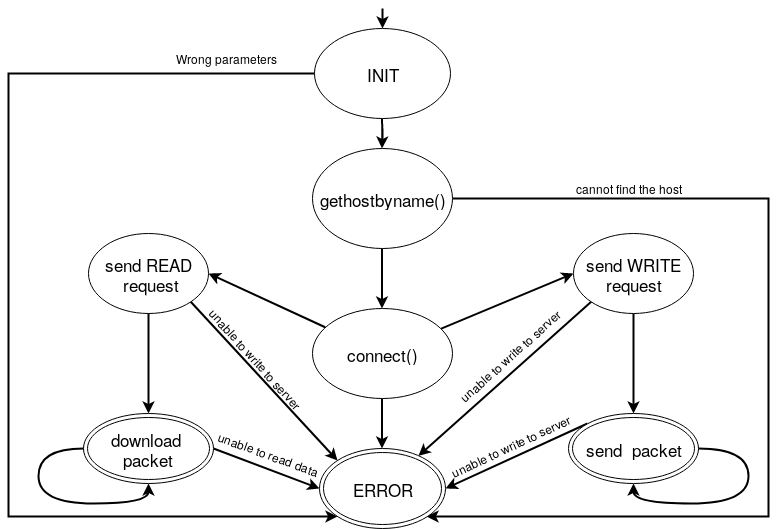
\includegraphics[scale = 0.5]{IPK_FSMKLIENT.png}


\section{Příklad použití}
\subsection*{strana klienta}
\textbf{\texttt{./ipk-client -h merlin.fit.vutbr.cz -p 20010 -r ./dir/filename.txt }}\\ \\
\texttt{INFO: connection establised}\\ \\
\texttt{INFO: directory "./dir/" was created}\\ \\
\texttt{INFO: file "filename.txt" was downloaded from server on address} \\  \texttt{merlin.fit.vutbr.cz}\\
\subsection*{strana serveru}
\textbf{\texttt{./ipk-server -p 20010}}\\ \\
\texttt{INFO: server inicialized and ready for connection(s) by client(s) }\\ \\
\texttt{INFO: new client connected from address 95.101.244.102}\\ \\
\texttt{INFO: file "filename.txt" sucessfuly sent to client (79.141.244.102)} \\ \\ 


\section{Zdroje informací}
\setlength\parindent{0pt}
[1] Computer Networking , A Top - Down Approach Featuring the Internet. 6. Polytechnic University, Brooklyn: Addison - Wesley, 2013. ISBN 9780132856201. \\

[2] Berkley sockets. In: Wikipedia: the free encyclopedia [online]. San Francisco (CA): Wikimedia Foundation, 2017 [cit. 2018-03-11]. \\Dostupné z: https://en.wikipedia.org/wiki/Berkeley\_socket\#saccept  \\

[3] C++ Tutorial : Sockets - Server \& Client - 2018 [online]. [cit. 2018-03-11]. Dostupné z: HONG, K. C++ Tutorial : Sockets - Server \& Client - 2018 [online]. 2018 [cit. 2018-03-11]. Dostupné z: http://www.bogotobogo.com/cplusplus/sockets\_server\_client.php







\end{document}